% !TeX root = ../main.tex
% ============================================================================
% Appendix F -- why the two tasks do not compete on the shared trunk.
%
% [round7, 2026-07-29] NEW APPENDIX, in the MAIN document at the author's request: "why these two
% tasks for our arch don't conflict and how this MAY be extended for others archs."
%
% IT IS THE LETTER F, after E, because Appendices B and D moved to the supplementary volume and the
% rest were NOT renumbered -- "Appendix B" already names the errata appendix outside this document.
% The A, C, E, F gap is deliberate; content.tex's appendix block carries the reasoning.
%
% CHAPTER 5'S BODY IS UNTOUCHED and does not point here. It is under review, so an edit for no
% reader benefit is not worth the divergence between the two texts.
%
% SOURCE OF RECORD FOR EVERY NUMBER: src_utils/_round7/gradient_cosine_observations.parquet (3,900
% rows; state, fold, epoch, cos, config) at commit ff69ba07, derived by _round7/cosine_stats.py,
% output quoted in _round7/24_extra_and_cosine.md. Re-derive, never increment: the count moved from
% three datasets to four mid-writing and every figure was recomputed at that point. If a fifth
% lands, re-run the script and read its output.
%
% TRAP -- THAT SCRIPT ONCE DID NOT RUN WHILE THIS FILE POINTED AT IT. It still declared 3 states /
% 3,650 rows after Georgia landed, so its own assertion killed it on the parquet it ships with. A
% file cannot be the source of record for numbers it refuses to compute; check that it runs (RC=0)
% before citing it. One value is NOT reproducible from the parquet alone: Alabama's "+0.058 over the
% first five epochs" is the mean of 25 values printed by the script's ALABAMA EPOCH BLOCKS section.
%
% TRAP -- THE UNIT OF INDEPENDENCE IS THE FOLD, and an earlier draft got this wrong. The 50
% per-epoch cosines within a fold are consecutive states of ONE trajectory. Every p-value is
% computed on fold means (n=5) or configuration means (Florida, n=12), never on the 3,900 raw
% observations, which would be anti-conservative.
%
% TRAP -- THE CLAIM A READER WILL WANT TO MAKE, AND MUST NOT. Alabama and Georgia are both 5/5
% positive with t-tests at p=0.0125 and p=0.0093. That is still not significance: the exact sign
% test returns 0.0625 for both, which IS its floor at n=5, so the rejection rests entirely on
% assuming normality. The same standard binds the downward-drift claim two paragraphs later -- they
% disagreed once, and 4445e7ab fixed it. Never write "significantly positive" here.
%
% COVERAGE: FOUR datasets (florida, alabama, arizona, georgia), ONE architecture family. California,
% Texas, and Istanbul are outstanding against job 805120f1, marked [VERIFY], and blocked on that
% host's disk rather than queued. Nothing here implies six datasets or any architecture coverage.
%
% [NEEDS SIGN-OFF: raised round 7, 2026-07-29 | THE WHOLE APPENDIX. New frame prose making a
% mechanistic claim (orthogonality explains why hard sharing costs nothing here) and a bounded
% extension claim. Neither is in any paper's claim whitelist, so both are new claims under
% AGENT_GUARDRAILS §3 C2 and need the author's approval before this goes to the advisor.]
% ============================================================================

\chapter{Why the Two Tasks Do Not Compete on the Shared Trunk}
\label{apx:cosine}

A joint model that shares parameters between two tasks can end up worse at both than two dedicated
models are at one each. The usual reason is a disagreement, and it shows up in the gradients: if the
update next-region asks for points against the update next-category asks for, one task improves at
the other's expense. That has a direct measurement, and this appendix runs it on the joint model of
Chapter~\ref{ch:mobiwac}.

The two tasks turn out not to disagree. Their gradients are statistically indistinguishable from
orthogonal on every dataset measured, which is a stronger and stranger result than mere absence of
conflict, and it carries a consequence for the whole investigation: a gradient balancer had nothing
to balance. That is why replacing the sharing scheme changed so little in the first study, and why
changing the representation changed so much in the second and third. The sections below give the
measurement, the two findings that qualify it, and the boundary beyond which none of it is claimed.

\section{What was measured, and on what unit}
\label{apx:cosine:setup}

At every training epoch, each task loss was back-propagated to the shared cross-attention trunk, and
the cosine of the angle between the two resulting gradient vectors was recorded. The cosine is the
right quantity because it is scale-free: it reads how the two requested updates are aligned and
ignores how large they are, which differs between the tasks and drifts during training. A cosine of
$+1$ means the tasks ask for the same update, $-1$ for opposite ones, and $0$ that the requests are
orthogonal, each leaving the other's objective unchanged to first order.

The observations are 3,900 epoch-level cosines from four datasets. Florida contributes 3,150 across
twelve configurations that vary the loss weight, the weighting schedule, and the training procedure;
Alabama, Arizona, and Georgia contribute 250 each at the canonical configuration. Every run is
five-fold user-disjoint cross-validation over fifty epochs, so one configuration on one dataset is
five series of fifty values, and two of Florida's carry a partial re-run on top of theirs.
% [round7, 2026-07-29] THE PARTIAL RE-RUN, previously undisclosed and now stated. "One
% configuration on one dataset is five series of fifty values" is true of 65 of the 75 series;
% T6_4_two_pass and T6_4_infonce_tau0_5 hold 65 rows per fold, because their epochs 1 to 15 each
% appear TWICE with different cosines. 10 series, 150 of the 3,900 rows. MEASURED:
%   df.groupby(['state','config','fold']).size().value_counts()  ->  50: 65 series, 65: 10 series
%   df[(df.state=='florida')&(df.config=='T6_4_two_pass')&(df.fold==1)].epoch.value_counts()
%     -> epochs 1..15 at count 2, epochs 16..50 at count 1
% IT DOES NOT TOUCH THE APPENDIX'S CLAIM and the prose does not imply that it might: both
% configurations remain equivalent to zero at the fold unit (TOST p=1.54e-05 and 2.90e-08), and
% deduplicating on (state, config, fold, epoch) moves the pooled mean +0.001182 -> +0.001526 and
% the within-margin share 91.28% -> 91.36%. It DOES move those two configuration means (two_pass
% -0.00261 -> -0.00055 keeping the first row of each duplicated epoch), and two_pass is the
% minimum of the reported span, so the span sentence in apx:cosine:extension is now explicit that
% it is computed over the rows as they stand. Understating a sentence's coverage silently is what
% GUARDRAILS 4b V2 forbids: a filter, a skip or a duplicate must be named with its count.

Three of the four, Florida, Alabama, and Arizona, are among the six Chapter~\ref{ch:mobiwac} reports
on. The fourth, Georgia, is a further Gowalla state the dissertation does not otherwise use; it
enters because the diagnostic ran on it cheaply and stays because dropping a measured dataset would
be a choice about the evidence. That chapter reaches the same conclusion from a smaller
development-time measurement, on an earlier data preparation and over four seeds rather than
per-epoch series, so the two sets of numbers are not interchangeable and this appendix supersedes
nothing there.
% [round7] THE SCOPE CORRECTION THAT MATTERS MOST IN THIS FILE. An earlier draft of this appendix
% called these "four datasets" without qualification, which would have told the reader that
% Georgia is one of the dissertation's six. It is NOT. MEASURED, from src/:
%   grep -v '^[[:space:]]*%' tables/mobiwac/datasets.tex | grep -E '^(AL|AZ|FL|TX|CA|Istanbul)'
%   -> AL, AZ, FL, TX, CA, Istanbul. Six rows. No Georgia.
% and Chapter 5's own related-work section says it outright: "and Georgia, which this
% dissertation does not otherwise use" (5_mobiwac/02_related.tex). So the appendix now says which
% three of its four datasets are the dissertation's and what the fourth is.
% THE OTHER HALF OF THE SAME PROBLEM: Ch.5's related-work paragraph ALREADY reports this cosine
% measurement, on these same four states, as averaging +0.001 with a largest per-dataset mean of
% +0.0032. My pooled mean over the 3,900 observations is +0.00118, close to its +0.001 -- but my
% largest per-dataset mean is Alabama's +0.0112, which is NOT its +0.0032. The two do not
% contradict each other because they are different runs (Ch.5's is development-time, four seeds,
% an earlier data preparation; this one is 5 folds x 50 epochs on the shipped preparation), but a
% reader who compared them without being told would read a discrepancy. Hence the sentence above.
% Chapter 5's prose is NOT edited: it is under review and its own numbers remain its own.

Those fifty values are not fifty independent measurements. They are consecutive states of one
training run, so treating them as independent draws would report more confidence than the data hold.
The unit of independence is the fold, and for Florida, whose twelve configurations reuse the same
five folds, the configuration. Every test below therefore runs on five fold means for Alabama,
Arizona, and Georgia and on twelve configuration means for Florida. Where a count of observations
appears it describes the data, not a test's sample size.
% [round7] "Alabama and Arizona" -> "Alabama, Arizona, and Georgia". Caught by READING THE
% RENDERED PAGE, not the source: the sentence was written when there were three datasets and the
% list was not revisited when Georgia landed, so the page named two datasets while the table below
% it listed four. A count updated in one place and not the other is AGENT_GUARDRAILS §4b V6.

Equivalence to zero is assessed by two one-sided tests against a margin of $\pm 0.05$
\cite{lakens2017tost}. The margin is a judgment about relevance and should be read as one: at
$|\cos| < 0.05$ one task's update projects less than five percent of its length onto the other's
direction, below the epoch-to-epoch variation in either gradient and below anything a balancing
method could act on. Chapter~\ref{ch:mobiwac}'s two-point margin for the region task measures a
different quantity on a different scale and should not be read against this one.
% [round7 review, 2026-07-29] THE MARGIN SENTENCES WERE MERGED INTO THIS PARAGRAPH. They used to be
% a separate paragraph after the comment block below, which left the citation sentence standing as a
% 13-word stub. Merging reads better and recovers a paragraph break's vertical space. The merge is
% done by moving the prose ABOVE the comment block rather than by deleting the blank line beneath it:
% deleting that blank line would also work, but the trapped-prose defect this file has already been
% bitten by lives exactly there, so the structural warning below stays true and unrelied-upon.
%
% [round7] CITATION KEY CORRECTED before this appendix ever appeared in a clean build. The
% first draft wrote \cite{lakens2017equivalence}, a key that does not exist in references.bib --
% invented from the author's name and the paper's topic, which is exactly the fabrication
% AGENT_GUARDRAILS §1 R1 forbids. The build caught it as one undefined citation. The real key,
% already used by Chapter 5 for the same procedure, is lakens2017tost (Lakens 2017, Soc.
% Psychol. Personal. Sci. 8(4):355-362, DOI 10.1177/1948550617697177), verified against the
% entry at references.bib rather than retyped. The appendix cites the same source Ch.5 does,
% which is what it should have done from the start.
%
% THE BLANK COMMENT LINE ABOVE, AND THE ONE BELOW THIS BLOCK, ARE LOAD-BEARING. A comment block
% that runs straight into a prose line makes TeX read the prose as a continuation of the comment,
% and the paragraph silently vanishes from the PDF with a clean build and no warning. That is
% science/AGENT_HANDOFF.md §2.1, the most persistent defect class in this repository, and it
% happened HERE: the margin-justification paragraph below was swallowed by the comment above and
% was absent from the rendered appendix until 2026-07-29. src_utils/check_trapped_prose.py is
% what caught it. End every comment block with a newline before prose resumes.

\section{The result}
\label{apx:cosine:result}

% !TeX root = ../../main.tex
% Table for Appendix F (apx_f_cosine.tex): the gradient-cosine equivalence result.
%
% EVERY CELL RE-DERIVED from src_utils/_round7/gradient_cosine_observations.parquet by
% src_utils/_round7/cosine_stats.py; its printed output is quoted in
% src_utils/_round7/24_extra_and_cosine.md. No cell is copied from a README or a brief.
%
% THE UNIT COLUMN IS NOT DECORATION. It names what n counts, because the 50 per-epoch cosines
% within a fold are one training trajectory and are not independent. Florida aggregates to
% configuration means (its 12 configurations reuse the same 5 folds); Alabama and Arizona to
% fold means. A p-value in this table without its unit is meaningless, which is why the unit
% and n sit in the same column group as the tests.
%
% ALABAMA'S t-TEST COLUMN IS DELIBERATELY ACCOMPANIED BY THE SIGN TEST AND ITS FLOOR. At n=5
% the exact sign test cannot return below 0.0625 even when all five values agree, so the
% t-test's 0.0125 rests entirely on normality at n=5. Reporting the t-test alone would present
% a suggestive pattern as an established effect; the floor column is what stops that reading.
\begin{table}[htbp]
    \centering
    \caption{The cosine between the next-region and next-category gradients on the shared
    trunk, on four datasets. Equivalence to zero is a two one-sided test (TOST) against a margin
    of $\pm 0.05$; it holds at every dataset, and the TOST column gives the order of magnitude of
    its $p$-value. Tests are computed on the independent unit named in the second column and
    never on the individual observations, because the fifty per-epoch values within a fold are
    one training trajectory rather than fifty independent draws; the observation count describes
    the data and is not the sample size of any test. Alabama and Georgia both show all five fold
    means positive with a $t$-test that rejects zero, but the exact sign test is at its floor at
    five observations, marked $\dagger$, so each is a consistent tendency rather than an
    established effect. Florida's unit is the configuration because its twelve configurations
    reuse the same five folds.}
    \label{tab:apx:cosine}
% WIDTH. Nine columns overflowed the text block by 132.49 pt in every build variant (measured:
% build.sh reported overfull_hbox=2 for DEFENSE and ACADEMICO, the first at "lines 33--45", which
% is this tabular). The header is now two-deep so the interval and the two floored tests fit in
% narrower columns, and the confidence interval is set as a single \makecell-free pair of short
% numbers. Re-measure after any column change; do not assume it still fits.
    {\small
    \setlength{\tabcolsep}{4pt}
    \begin{tabular}{llrrlrrr}
        \toprule
        & & \multicolumn{2}{c}{Sample} & \multicolumn{2}{c}{Mean cosine} & \multicolumn{2}{c}{$p$ against zero} \\
        \cmidrule(lr){3-4}\cmidrule(lr){5-6}\cmidrule(lr){7-8}
        Dataset & Unit & $n$ & obs. & 95\% CI & mean & TOST & $t$ / sign \\
        \midrule
        Florida & configuration & 12 & 3{,}150 & $[-0.0012, +0.0017]$ & $+0.0003$ & $10^{-16}$ & $0.70$ / $0.77$ \\
        Alabama & fold          &  5 &   250 & $[+0.0040, +0.0184]$ & $+0.0112$ & $10^{-5}$  & $0.013$ / $0.063^{\dagger}$ \\
        Arizona & fold          &  5 &   250 & $[-0.0051, +0.0081]$ & $+0.0015$ & $10^{-5}$  & $0.56$ / $1.00$ \\
        Georgia & fold          &  5 &   250 & $[+0.0016, +0.0061]$ & $+0.0039$ & $10^{-7}$  & $0.009$ / $0.063^{\dagger}$ \\
        \bottomrule
        \multicolumn{8}{l}{\footnotesize $^{\dagger}$ $0.0625$ is the smallest value the exact sign test can return at $n = 5$.} \\
    \end{tabular}
    }
\end{table}


Every dataset is equivalent to zero, and Table~\ref{tab:apx:cosine} gives each one's mean, confidence
interval and tests. All four means lie within one and a half hundredths of zero, against a margin of
five hundredths, and equivalence holds at every other level of aggregation as well, including the raw
observations, so the conclusion does not depend on the choice of unit.
% [round7] THE PER-DATASET NUMBERS WERE MOVED OUT OF THIS PARAGRAPH INTO THE TABLE, for two
% reasons that coincided. (1) They were duplicated: every value here was already in
% tables/frame/cosine.tex, so a correction had to be made twice or the two would disagree.
% (2) Five inline math intervals in running prose gave TeX nothing to break on and produced an
% overfull hbox of 5.48 pt (measured: build.sh, "lines 111--118"). The prose now says what the
% numbers mean and the table carries the numbers, which is the arrangement WRITING_LAW §5 asks
% for anyway (a results table introduced by a lead takeaway sentence).

The distance between that result and a null result is the point of this appendix. A test that merely
failed to reject zero would license one statement, that no conflict was detected, which is equally
consistent with a conflict too small to see at this sample size. An equivalence test licenses the
positive claim instead: the mean alignment lies inside a margin fixed in advance, so whatever
alignment is there is too small to matter. That is a claim about the tasks, not about the
experiment's power.

Figure~\ref{fig:apx:cosine} shows the distributions, and one feature needs saying plainly: the
equivalence is a statement about the mean, not about every observation. Of the 3,900 cosines, 91.3
percent fall inside the margin, and the full range runs from $-0.34$ to $+0.58$, the largest value
lying past the right edge of panel (a). Individual epochs drift out of the margin in both
directions, ordinary noise in a quantity computed from one mini-batch. What never happens is a
systematic pull to one side.

\begin{figure}[htbp]
    \centering
    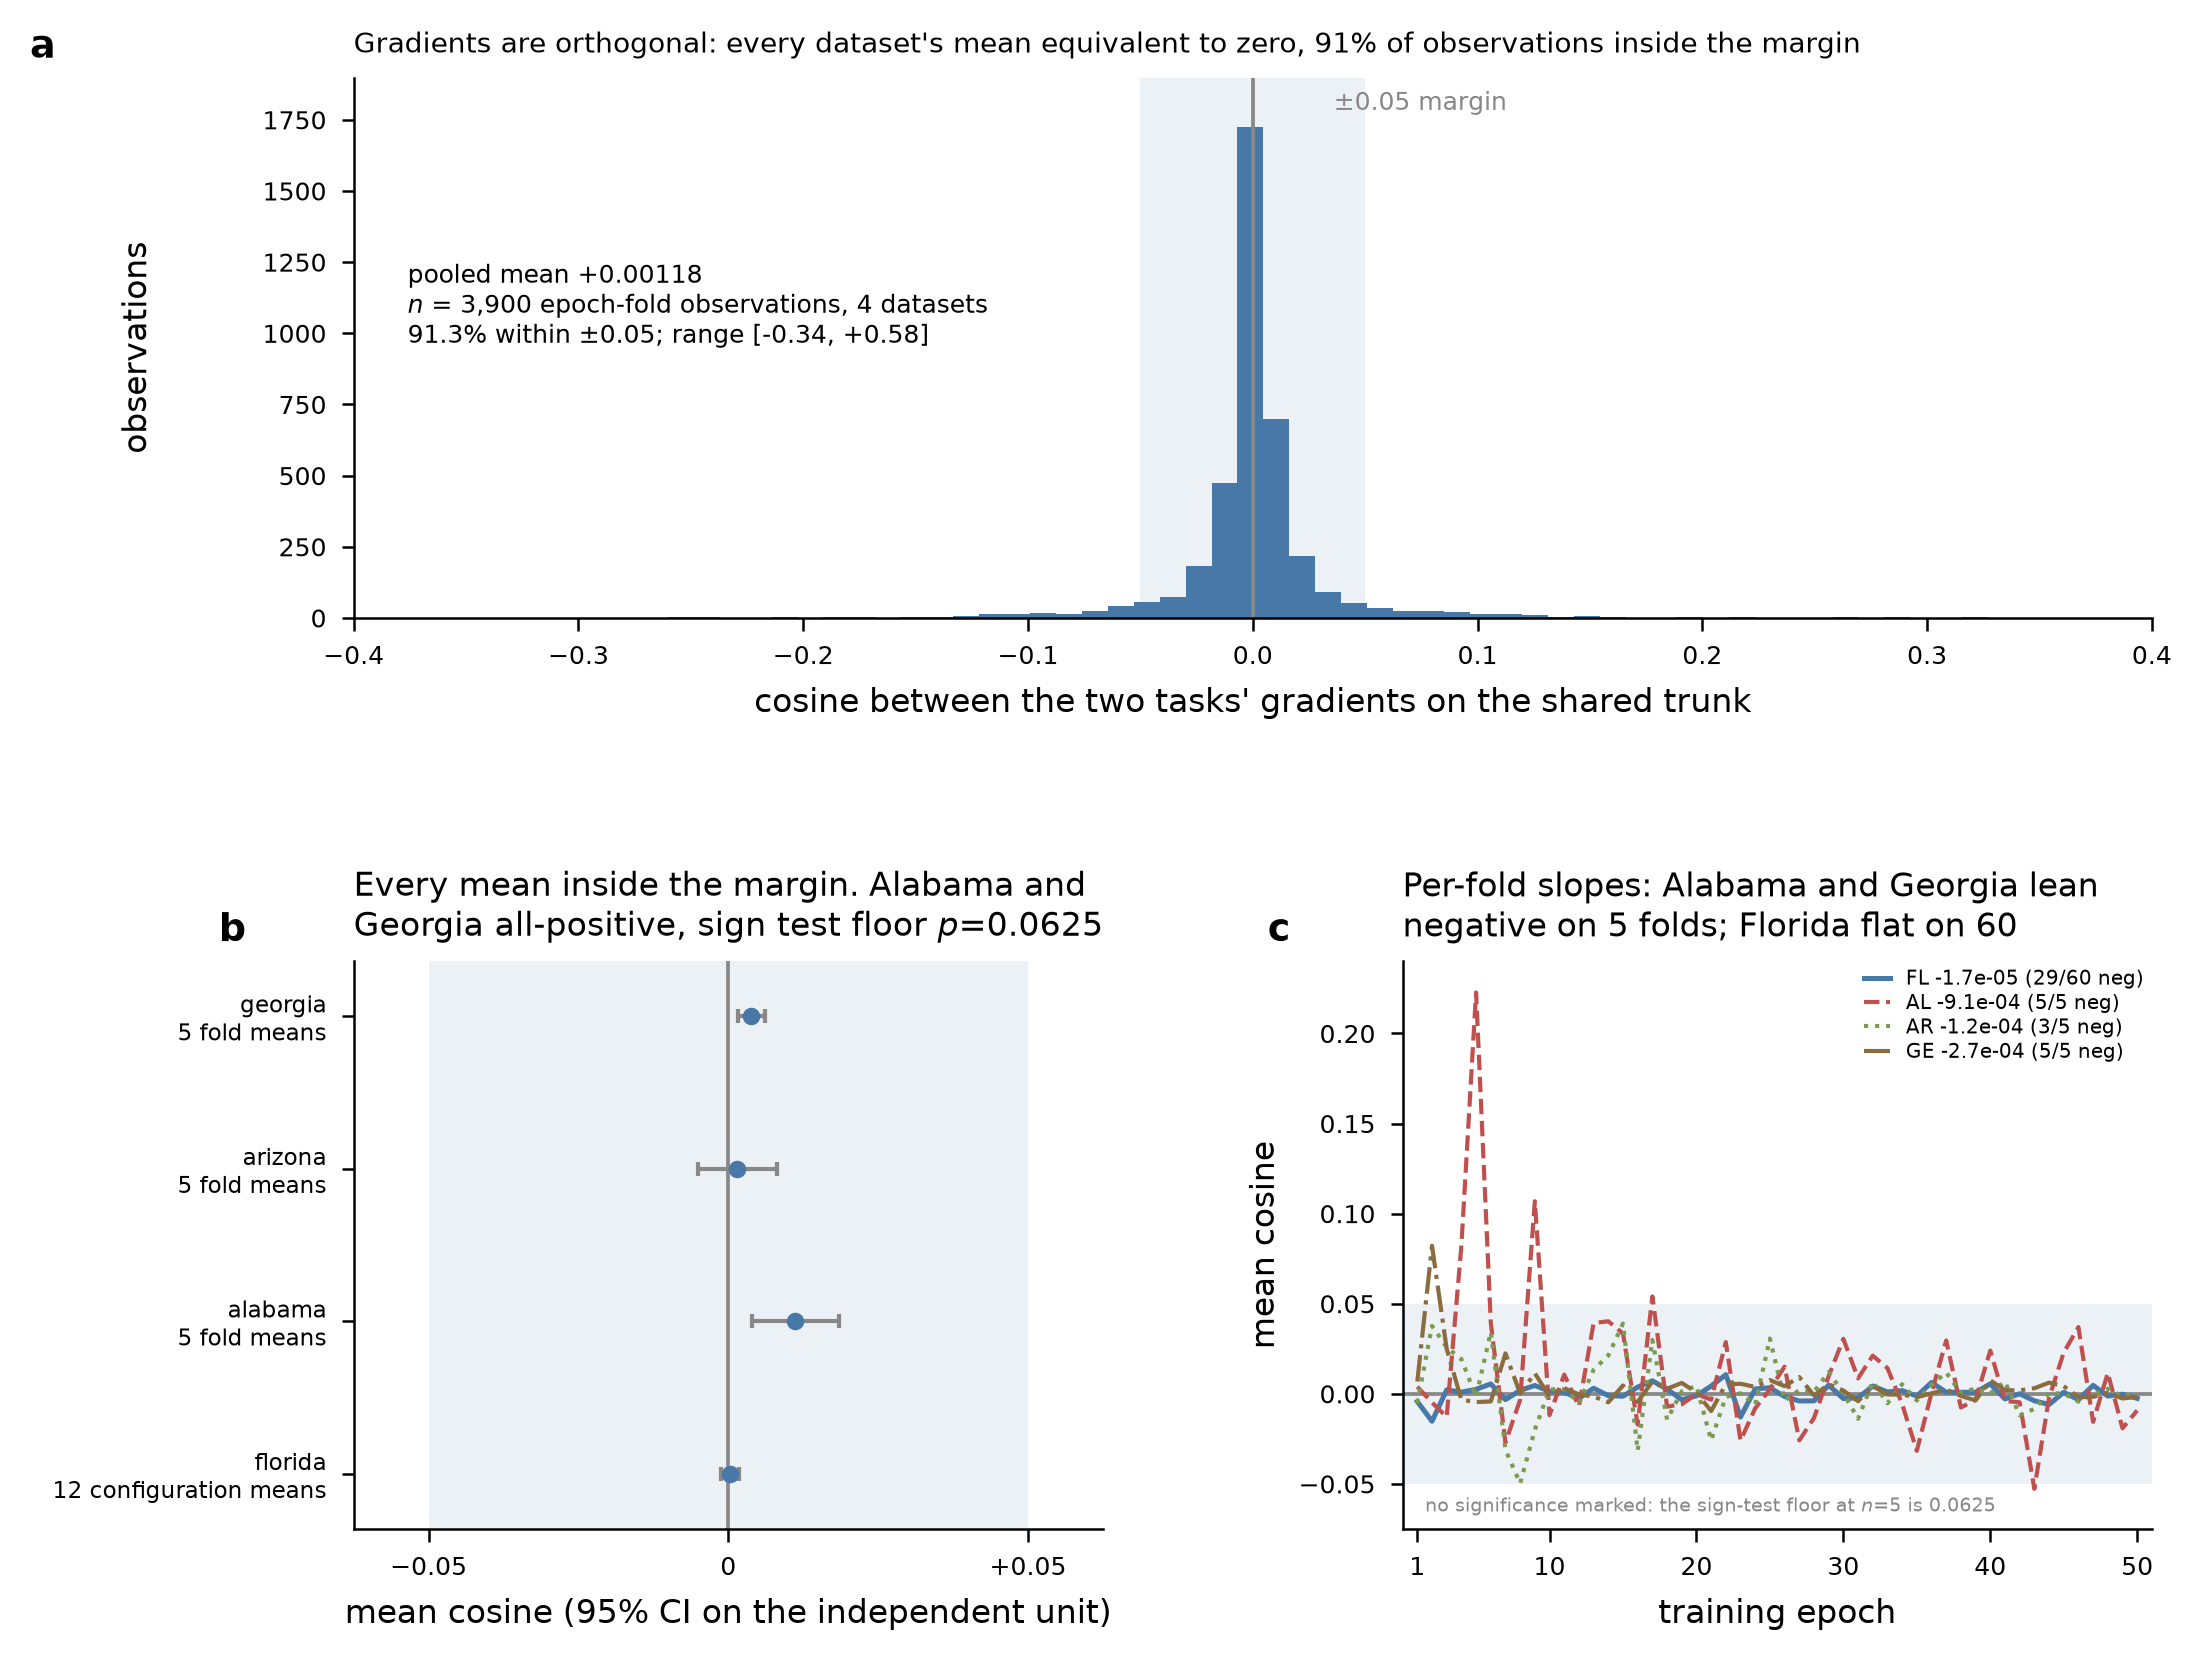
\includegraphics[width=\textwidth]{figures/fig_gradient_cosine}
    \caption{The two tasks' gradients on the shared trunk are orthogonal, on four datasets.
    The shaded band is the equivalence margin of $\pm 0.05$; every mean falls inside it. Panels:
    (a) the pooled distribution, (b) each dataset's mean with its 95 percent interval, (c) the
    mean over training. No significance is marked anywhere in the figure.}
    \label{fig:apx:cosine}
% [round7, 2026-07-29] THE CAPTION WAS 199 WORDS AND THREE OF ITS STATEMENTS WERE FALSE. It
% described the PRE-GEORGIA figure: commit 4445e7ab rebuilt the image from the four-dataset
% parquet and fixed the caption's panel-(c) sentence, but nobody re-read its panel-(a) sentence
% against the new render. AGENT_GUARDRAILS 4b V6 again -- corrected in one place, stale in
% another. All three defects were MEASURED FROM THE PNG's pixels, not judged by eye:
%   1. "one outline per dataset, with the number of observations in the key" -- panel (a) is ONE
%      POOLED histogram. Exactly one blue RGB triple (72,120,168) occurs in its plot area and
%      there is no per-dataset key; its in-panel annotation reads "n = 3,900 epoch-fold
%      observations, 4 datasets". The per-dataset lines are panel (c), which has four.
%   2. "the dashed line marks zero" -- it is SOLID. The column at cosine 0 carries grey in 539 of
%      the 562 plot rows and every row-gap is 1 px. Nothing about the render is dashed.
%   3. "the horizontal axis is clipped at +/-0.20 ... so the tails reaching -0.34 and +0.58 are
%      outside the frame" -- the axis runs -0.40 to +0.40 (ticks measured at 224 to 225 px per
%      0.10 unit), so -0.34 is INSIDE the frame and visible. Exactly ONE observation of 3,900
%      (+0.5802) lies beyond the axis, which is what the caption now says. 99.97% of the data is
%      within the drawn range.
% WHAT WAS CUT AND WHERE IT LIVES: the 91.3 percent and the -0.34/+0.58 range (body, the
% paragraph introducing this figure), the twelve-configurations/five-folds spelling out of the
% independent unit (Section apx:cosine:setup and the table caption), and the sign-test-floor
% explanation (stated in full in the drift paragraph). Nothing was lost, and per WRITING_LAW §5
% the caption still names every element and carries its reading instruction.
\end{figure}

Two departures from that flat picture appear on the smaller datasets, and both are worth reporting
rather than smoothing. The first is a positive tendency that recurs: all five of Alabama's fold means
are positive, averaging $+0.0112$, and so are all five of Georgia's, averaging $+0.0039$. The second
is a decline over training, on the same two datasets and with the same unanimity, all five per-fold
slopes negative in each; Arizona is mixed at three of five, and Florida is flat.

Neither is called significant here, and the reason is the design rather than the data. At five folds
the exact sign test cannot return less than $0.0625$, so no distribution-free test could reach
significance however consistent the pattern. A $t$-test does reject in all four cases, but at five
observations that rests entirely on assuming normality, and this appendix will not accept for one
claim a basis it rejects for another. Both are therefore consistent tendencies rather than
established effects. Florida, whose sixty independent series are the only estimate in the set with
the resolution to settle either question, shows neither.

Both point away from trouble in any case. A positive cosine is mild cooperation, not conflict, and
the decline stays inside the margin throughout while moving toward zero rather than away from it. No
mechanism is proposed for either.
% [round7] "Alabama and Georgia are the smallest datasets here" was CUT as unsourced. Alabama is
% indeed the smallest of the dissertation's six (113,846 check-ins, tables/mobiwac/datasets.tex),
% but Georgia is not in that table at all -- it is not one of the six -- so no committed artifact in
% this repository states its size, and I did not measure it. The sentence now says what IS
% measurable from the observations themselves: both estimates rest on five folds against Florida's
% sixty series. Same point about precision, no unverifiable size claim.

\section{What orthogonality explains}
\label{apx:cosine:mechanism}

Orthogonal gradients mean neither task's update reinforces or cancels the other's on the shared
parameters, so the trunk can serve both without either improvement being paid for by the other. Two
consequences follow.

The first is about gradient balancers. Nash-MTL and the family around it exist to resolve exactly
the disagreement measured here, reweighting or reprojecting task gradients so a dominant task cannot
overwrite a weaker one. Orthogonality leaves them nothing to resolve. That is why hard sharing costs
nothing in this architecture, and why Chapter~\ref{ch:mobiwac} finds no balancer improving on a
fixed loss weighting: the measurement explains the finding.

The second is about the arc of the three studies. The investigation opened on the hypothesis that
the sharing scheme limited joint training, and the first study's null result was read that way at
the time. Had the tasks been in conflict, a better sharing scheme or a better balancer would have
been the remedy. They were not, so the limit lay elsewhere, and the second and third studies located
it in the input representation. There was little interference to fix, and therefore little for a
change of architecture to recover.

\section{How far this extends, and how far it does not}
\label{apx:cosine:extension}

Four datasets and twelve configurations bound this result along two axes, each answering a different
objection.

The first axis is the tuning. Every one of Florida's twelve configurations is equivalent to zero on
its own five folds, and their twelve means span $[-0.00261, +0.00457]$ over the observations as
recorded. Orthogonality survives every hyperparameter and procedure that was varied, so it is not an
artifact of one choice among them.
% [round7] SPAN CORRECTED before first build: this read [-0.00214, +0.00457], which is the
% SECOND-lowest configuration mean (T6_1_lambda0_2). The minimum is -0.00261 (T6_4_two_pass).
% Read from cosine_stats.py's "configuration-mean span" line, which exists to be quoted.
% "equivalent to zero on its own five folds" is also measured, not asserted: that script's
% per-configuration block reports 12 of 12 equivalent at the fold unit.
The second axis is the data. Among the three datasets Chapter~\ref{ch:mobiwac} also reports, the
check-in counts run from 113,846 at Alabama to 1,407,034 at Florida and the region counts from
1,109 to 4,703, so this axis spans an order of magnitude in volume, and Georgia adds a fourth
state under the same protocol. The result is not a quirk of Florida either.

Together the two axes suggest orthogonality belongs to the task pair rather than to the tuning. Next
category asks which of seven kinds of place a user visits next, next region asks which tract or
neighborhood, and both read the same trace to predict a different projection of one event. Those
projections appear close to statistically independent given the shared representation, which would
explain why each task's update carries so little of the other's.

That is where the evidence stops, and the boundary matters. Every run measured here uses one
architecture family, the cross-attention joint model of Chapter~\ref{ch:mobiwac}. The architecture
decides where the two tasks meet and how much they share, which makes it at once the factor most
likely to change the answer and the one this appendix did not vary. Nothing here says the gradients
stay orthogonal in a model that shares more of its depth, couples the tasks in a cascade, or shares
an output layer. Settling that needs the same diagnostic and nothing else changed: the per-epoch
cosine on the candidate's shared parameters, under a fixed loss weighting, across one dataset's
folds, with the fold means tested for equivalence against a margin chosen in advance. Equivalence
there makes orthogonality the task pair's property; otherwise it belongs to this architecture, and
Section~\ref{apx:cosine:mechanism} applies only to models shaped like this one.

California, Texas, and Istanbul, the other three datasets of Chapter~\ref{ch:mobiwac}, are missing
above for reasons of computational resource rather than of principle. California and Texas are the
two largest of the six and the region task at that scale forces full single-precision training, and
the attempt ran out of disk on the machine that would have done it; Istanbul, a smaller dataset, was
queued behind them when the disk filled. The diagnostic needs no new method, so what these three lack
is the run itself rather than a way to perform it. The coverage here is therefore three
of the dissertation's six datasets plus Georgia, and a reader should not extrapolate to the rest.
% [NEEDS SIGN-OFF: PENDENCIAS 2.9, round8, 2026-07-30] ONE CLAUSE REPLACED, AND THE REASON IS THAT
% IT HAD BECOME FALSE. It read "so all three are blocked on that machine's free space rather than
% waiting in its queue". That was a PRESENT-TENSE claim about a remote machine, and a remote state
% verified once does not stay true -- the same lesson PENDENCIAS 2.1 records about origin/mobiwac.
% Re-measured 2026-07-30T00:48Z over ssh:nespedgpu, `df -h /home`:
%     /dev/mapper/vg0-home  393G  313G  61G  84% /home
% 61G free, not 0. results/check2hgi/california/checkpoints (the 61G this comment names below) is
% ABSENT; that whole state directory is now 64M. The author freed it -- "DECISAO: Liberado" in
% PENDENCIAS 2.9 -- so the sentence outlived its own measurement by a day.
% The replacement clause is true whether or not the runs are ever made, and it says the same thing
% to the reader: the gap is a run, not a method. WHETHER TO MAKE THE RUN IS THE AUTHOR'S CALL and is
% recorded as its own decision in PENDENCIAS 2.9 with the measured cost; nothing here presumes it.
% The two sentences before this one are HISTORY and stay: the attempt really did run out of disk.
% [round7, 2026-07-29] DO NOT WRITE "the largest of the six" ABOUT THESE THREE. It is false for
% Istanbul, which is the SMALLEST by region count and smaller than Florida, which IS measured here.
% Measured from tables/mobiwac/datasets.tex (strip comments first, the table has them):
%   check-ins: AL 113,846 | AZ 236,450 | ISTANBUL 462,615 | FL 1,407,034 | CA 3,171,380 | TX 4,089,892
%   regions:   Istanbul 520 | AL 1,109 | AZ 1,547 | FL 4,703 | TX 6,553 | CA 8,501
% The size claim is therefore scoped to California and Texas; Istanbul's reason is that it never
% started.
% [SUPERSEDED 2026-07-30, round8] This paragraph used to end: 'Say BLOCKED, never "pending" or
% "queued": PENDENCIAS §2.9 measures the host at 0 bytes free, so these runs cannot start, and a
% reader told they are queued is being told something false.' THE DISK IS NO LONGER FULL (61G free,
% measured 2026-07-30T00:48Z; see the sign-off note at the coverage paragraph), so that instruction
% now tells the next agent to write something false, which is the exact failure it was written to
% prevent. Superseded rather than deleted, per AGENT_GUARDRAILS §4b V5: an instruction that expired
% is evidence about how this file drifts, and a reader who finds only its absence learns nothing.
% WHAT TO SAY NOW: say the runs were NOT MADE, and do not attribute the gap to any live condition on
% the host without re-running `df -h /home` in the same session and dating the reading.
% [VERIFY: the per-dataset extension to California, Texas, and Istanbul. STATUS at the time this
% appendix was written, from the job's own _status.json and not from its log: job 805120f1 on
% ssh:nespedgpu was KILLED by SIGTERM at a 35-minute wall-clock cap (exitCode 124 at 35.0 min).
% It completed alabama, arizona and georgia -- which is where three of this appendix's four
% datasets come from -- and was cut off inside california's fold 1; texas and istanbul never
% started. Texas and Istanbul were resubmitted as separate single-dataset jobs c2a02f5d and
% d332e69e, and California as five per-fold jobs (213ce119 for the retry).
%
% THE RUN IS BLOCKED, NOT PENDING, and the blocker is not compute. The GPU host's disk is FULL:
% 373G of 393G used, 0 bytes available. That is what California actually died of --
% "RuntimeError: basic_ios::clear: iostream error" is a failed WRITE, not a model failure -- and
% two folds produced no output while their job still exited 0, which is the "well-formed output
% carrying no data" shape of AGENT_HANDOFF §2.7. The space is pre-existing and belongs to other
% work (61G in results/check2hgi/california/checkpoints; PoiMtlNet totals 94G); the diagnostic
% runs themselves are about 15 MB. Freeing it is the author's decision and nothing was deleted.
% ALSO DO NOT TRUST CALIFORNIA'S FOLDS 2 AND 3 IF YOU FIND THEM ON DISK: they were harvested by
% a step that resolves the newest output directory, which races under concurrent jobs, and
% "--only-fold k" writes its output as fold1_diagnostics.csv for every k, so the filename carries
% no fold identity. The two files are byte-identical and cannot be attributed to a fold by any
% evidence on disk. Using them would put a duplicated fold in a dissertation appendix.
% This is why the appendix stops at four datasets: a coverage sentence naming a dataset whose
% observations are not in the parquet is the defect that caution exists to avoid.
% THREE ESTIMATION ERRORS ARE RECORDED HERE BECAUSE EACH WOULD HAVE REACHED THIS FILE, and they
% share one lesson -- derive a runtime from the thing's OWN timestamps. (3) is the newest: California
% was priced at 1.49 min/epoch by dividing the WHOLE JOB's elapsed time, which already covered
% alabama, arizona and georgia, by california's own 34 epochs; from its own start and kill stamps the
% rate is 0.446 min/epoch, about 22 min per fold. A 3.3x error, and the difference between
% "impossible under the cap" and "one fold fits easily". No runtime figure appears in the prose
% above, deliberately: a runtime is not a result, and each of these was wrong before it was right.
% (1) Georgia was estimated at 8.7 h from its FIRST epoch and finished in 11 minutes, a 47x error,
% because epoch 1 carries warmup -- never extrapolate a run from its first epoch. (2) California was
% reported as "about 5.4 h remaining" for a process that was already dead: its log had been frozen
% for 78 minutes and the GPU was idle, and the stale log was being read as progress. Check the
% process, not the log.
% WHEN THE RUNS LAND: re-run src_utils/_round7/cosine_stats.py (it asserts its own structure),
% extend tables/frame/cosine.tex and rebuild the figure, then correct EVERY count in this file.
% The dataset count appears in: this file's header comment (twice), the observations paragraph,
% the "three of those four" paragraph, the figure caption, the table caption, the first sentence
% of Section apx:cosine:extension, the data-axis paragraph, and the paragraph above. Grep for
% "3,900", "four datasets" and "3,150 + 250" rather than trusting this list to stay complete.]
